% !TEX program = xelatex

\documentclass[10pt,aspectratio=169,mathserif]{beamer}
%设置为 Beamer 文档类型,设置字体为 10pt,长宽比为16:9,数学字体为 serif 风格

%%%%-----导入宏包-----%%%%
\usepackage{ecnu}			%导入 CCNU 模板宏包
\usepackage{ctex}			 %导入 ctex 宏包,添加中文支持
\usepackage{amsmath,amsfonts,amssymb,bm}   %导入数学公式所需宏包
\usepackage{color}			 %字体颜色支持
\usepackage{graphicx,hyperref,url}
\usepackage[most]{tcolorbox}
\usepackage{colortbl}
\usepackage{geometry}
\tcbuselibrary{skins, breakable, theorems, fitting}

%%%%%%%%%%%%%%%%%%

%%%%%%%%%%%%%%%%%%

\beamertemplateballitem		%设置 Beamer 主题

\setbeamertemplate{navigation symbols}{}		% 取消右下角导航栏

%%%%------------------------%%%%%
\catcode`\。=\active         %或者=13
\newcommand{。}{.}				
%将正文中的“。”号转换为“.”。
%%%%%%%%%%%%%%%%%%%%%

%%%%----首页信息设置----%%%%
\title[Design and Implementation of Othello Based on Reinforcement Learning]{基于强化学习的黑白棋的设计与实现}
\subtitle{Design and Implementation of Othello Based on Reinforcement Learning}			
%%%%----标题设置


\author[by im0qianqian]{
  Zhao Qian \\\medskip
  {\small {Adviser: Jerry Wang}} \\
}
%%%%----个人信息设置

\institute[YTU]{
  Yantai University \\
  School of Computer and Control Engineering}
%%%%----机构信息

\date[2019.05.30]{
  2019.05.30}
%%%%----日期信息

\begin{document}

\begin{frame}
\titlepage
\end{frame}				%生成标题页

\section{大纲}
\begin{frame}
\frametitle{Outline}
\tableofcontents[]
\end{frame}				%生成提纲页


\section{研究动机}
\begin{frame}
  \frametitle{Why Reversi and Prior Work}
	\begin{columns}
    \column{.55\textwidth}
      \begin{tcolorbox}[standard jigsaw,title=Why Reversi?,height=6.5cm,opacityback=.5,colbacktitle=black!70!white,colframe=white]
      % \begin{block}{Why Reversi?}
				\begin{figure}[tb]
			        \centering
			        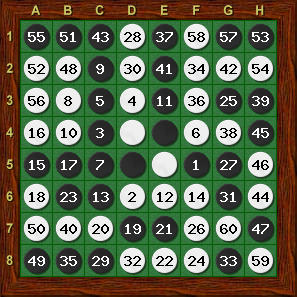
\includegraphics[width=.5\textwidth]{img/othello.jpg}
			    \end{figure}
				\begin{footnotesize}
					\begin{itemize}
						\item {\songti 以往算法的设计中大都使用博弈树搜索的方法}
						\item {\songti 2017 年 AlphaGo Zero 出现了}
						\item {\songti 打算将这种思路扩展到黑白棋中}
					\end{itemize}
        \end{footnotesize}
      % \end{block}
			\end{tcolorbox}
    \column{.55\textwidth}
    \begin{tcolorbox}[standard jigsaw,title=Prior Work,height=6.5cm,opacityback=.5,colbacktitle=black!70!white,colframe=white]
      % \begin{block}{Prior Work}
        \begin{footnotesize}
          \textbf{Minimax Tree Search + Alpha-Beta pruning}
						\begin{itemize}
							\item {\songti 搜索空间巨大(随搜索层数指数级增加)}
							\item {\songti 棋力受限于搜索的层数(理想时间内很难提高)}
							\item {\songti 棋力受限于设计者的能力(如估值函数的设计)}
            \end{itemize}
          \vspace{1cm}
          \textbf{Monte Carlo Tree Search}
          \begin{itemize}
							\item {\songti 无需任何领域知识便可工作}  % MCTS 不要求任何关于给定的领域策略或者具体实践知识来做出合理的决策。这个算法可以在没有任何关于博弈游戏除基本规则外的知识的情况下进行有效工作;这意味着一个简单的 MCTS 实现可以重用在很多的博弈游戏中,只需要进行微小的调整,所以这也使得 MCTS 是对于一般的博弈游戏的很好的方法。
							\item {\songti 非对称式增长,算法会频繁地访问“更感兴趣”的节点,并聚焦搜索空间于更加相关树的部分}
							\item {\songti 算法可在任何时间终止,并返回当前最优的估计}
					\end{itemize}
        \end{footnotesize}
      % \end{block}
			\end{tcolorbox}
	\end{columns}
\end{frame}

\section{游戏规则}
\begin{frame}
  \frametitle{Reversi: Basic Rules}
  \begin{columns}
    \column{.55\textwidth}
    \begin{tcolorbox}[standard jigsaw,title=How to play,height=6.5cm,opacityback=.5,colbacktitle=black!70!white,colframe=white]
        \begin{minipage}[b]{0.30\textwidth}
          \flushleft
          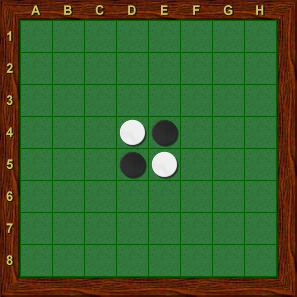
\includegraphics[height=1.0\textwidth]{img/othello_init.jpg}
        \end{minipage}
        \begin{minipage}[b]{.65\textwidth}
          \flushright
          \begin{footnotesize}
            \begin{itemize}
              \item {\songti 棋盘 $8 \times 8$ 大小}
              \item {\songti E4、D5 为黑棋}
              \item {\songti D4、E5 为白棋}
              \item {\songti 执黑先手}
            \end{itemize}
            \medskip
          \end{footnotesize}
        \end{minipage}
        \tcblower
        \begin{minipage}[b]{.55\textwidth}
          \flushleft
          \begin{footnotesize}
            \begin{itemize}
              \item {\songti 落子必须在一空位}
              \item {\songti 落子必须造成翻转}
              \item {\songti 无子可走则本轮 pass}
              \item {\songti 有子可走则必须走棋}
            \end{itemize}
          \end{footnotesize}
          \medskip
        \end{minipage}
        \begin{minipage}[b]{0.4\textwidth}
          \flushright
          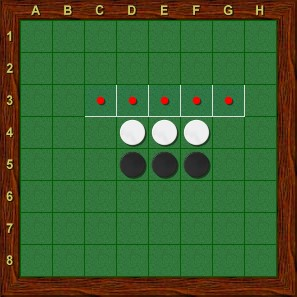
\includegraphics[height=1.0\textwidth]{img/othello1.jpg}
        \end{minipage}
    \end{tcolorbox}
    \column{.55\textwidth}
    \begin{tcolorbox}[standard jigsaw,title=How to win,height=6.5cm,opacityback=.5,colbacktitle=black!70!white,colframe=white]
      \begin{figure}[tb]
        \centering
        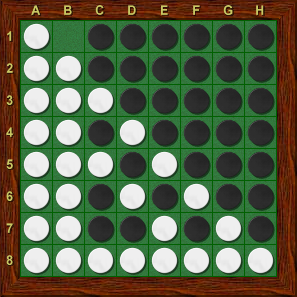
\includegraphics[width=.5\textwidth]{img/othello_end.jpg}
      \end{figure}
      \begin{footnotesize}
        \small \textbf{获胜条件:}
        \begin{enumerate}
          \item \songti 双方都无子可下
          \item \songti 棋子数目多者获胜,若相等为平局
        \end{enumerate}
      \end{footnotesize}
    \end{tcolorbox}
  \end{columns}
\end{frame}

\section{强化学习}
\begin{frame}
  \frametitle{Reinforcement Learning}
	\textbf{Sample Text...。。。\\}
	\noindent\textbf{Sample Text\\}
\end{frame}

\section{系统设计}

\subsection{整体架构}
\begin{frame}
  \frametitle{Structure Breakdown}
	\textbf{Sample Text\\}
	\noindent\textbf{Sample Text\\}
\end{frame}

\subsection{兼具策略评估与价值评估的神经网络}
\begin{frame}
  \frametitle{Neural Policy and Value Network}
	\textbf{Sample Text\\}
	\noindent\textbf{Sample Text\\}
\end{frame}

\subsection{使用蒙特卡洛搜索进行策略改进}
\begin{frame}
  \frametitle{Monte Carlo Tree Search for Policy Improvement}
	\textbf{Sample Text\\}
	\noindent\textbf{Sample Text\\}
\end{frame}

\section{实验分析}
\begin{frame}
  \frametitle{Experiments and Analysis}
	\textbf{Sample Text\\}
	\noindent\textbf{Sample Text\\}
\end{frame}


\section{总结展望}
\begin{frame}
  \frametitle{Conclusions and Prospect}
  \noindent\textbf{Sequence Tagging Loss\\}
    \[{\mathcal{L}_p} =  - \sum\limits_{i = 1}^S {\sum\limits_{j = 1}^N {{p_{i,j}}\log ({{\hat p}_{i,j}})} } \]
  \noindent\textbf{Language Classifier Loss\\}
   \[{\mathcal{L}_a} =  - \sum\limits_{i = 1}^S {{l_i}\log ({{\hat l}_i})}\]
  \noindent\textbf{Bidirectional Language Model Loss\\}
   \[{\mathcal{L}_l} =  - \sum\limits_{i = 1}^S {\sum\limits_{j = 1}^N {\log (P({w_{j + 1}}|{f_j})) + \log (P({w_{j - 1}}|{b_j}))} }\]
\end{frame}

\section{致谢}
\begin{frame}{Acknowledgement}
  \begin{itemize}
    \item {\heiti 感谢王建华老师在毕设期间的指导}
    \item {\heiti 感谢 ACM 实验室 卢云宏老师、周世平老师、封玮老师}
    \item {\heiti 感谢班主任毕远伟老师}
    \item {\heiti 感谢四年里遇到的各位老师和同学}
  \end{itemize}
  \medskip
  \begin{center}
    \LARGE \textbf{请多提宝贵意见}
  \end{center}
\end{frame}

\end{document}
